\documentclass{article}

\usepackage[preprint]{neurips_2025}

\usepackage[utf8]{inputenc}
\usepackage[T1]{fontenc}
\usepackage{hyperref}
\usepackage{url}
\usepackage{booktabs}
\usepackage{amsfonts}
\usepackage{amsmath}
\usepackage{graphicx}
\usepackage{natbib}
\usepackage{microtype}
\usepackage{placeins}

\title{Reproducing PhyCustom on FLUX: An Empirical Reproduction Study}

\author{Anonymous Author(s)}

\begin{document}

\maketitle

\begin{abstract}
Reproducing physically grounded customization methods on newer text-to-image backbones remains difficult because apparent gains can depend on implementation details as much as on the underlying intervention principle. This issue is especially important for FLUX, whose architecture and tuning behavior differ from the setting in which PhyCustom was introduced \cite{wu2025phycustom,blackforestlabs2024fluxdev}. We present a reproduction protocol for transferring PhyCustom-style customization to FLUX through lightweight adapters, prompt-swapped comparisons, and consistency constraints, while explicitly framing the study as reproduction rather than a new method proposal. The current evidence supports a narrow empirical conclusion: we implemented the FLUX-side reproduction scaffold, mapped the original intervention idea to five planned adaptation variants, and established the evaluation axes and qualitative criteria needed for comparison, but the available validated artifact contains one recorded execution and no finalized metric outputs. This outcome shifts the paper from a completed benchmark comparison to a reproduction report centered on protocol design, implementation fidelity, and what remains necessary for a fully validated empirical comparison. The main takeaway is that reproducing PhyCustom on FLUX is a well-posed and technically meaningful target, but claims about superiority, significance, or realism--fidelity trade-offs require regenerated result artifacts that match the implemented protocol.
\end{abstract}

\section{Introduction}

Customization is one of the most practically important capabilities in text-to-image generation because users rarely want generic synthesis; they want a model to preserve a specific subject, appearance attribute, or physically meaningful property while still responding to new prompts. That requirement has driven a large body of work on personalization, subject-driven generation, concept injection, and parameter-efficient tuning for diffusion and related generators \cite{ruiz2023dreambooth,kumari2023multiconcept,hu2021lora}. Yet a central question now extends beyond whether a customization method works in its original codebase. As model families diversify, the more consequential question is whether the intervention principle transfers across backbones with different conditional pathways, latent parameterizations, and optimization behavior. This issue is especially acute for physically grounded customization, where success depends not only on visual resemblance but on preserving a structured intervention under prompt variation \cite{wu2025phycustom,blackforestlabs2024fluxdev}. Reproducing PhyCustom on FLUX is therefore a focused test of algorithmic portability: does the core intervention idea survive migration to a newer backbone, or were the original gains partly tied to framework-specific details?

That gap is not resolved by prior customization literature. DreamBooth and related personalization methods showed that small reference sets can induce strong subject retention in diffusion models \cite{ruiz2023dreambooth,kumari2023multiconcept}. Textual inversion and follow-up adapter methods demonstrated that low-dimensional or low-rank updates can encode concept information while preserving much of the pretrained generator \cite{hu2021lora}. At the same time, work on diffusion reproducibility and evaluation has shown that generative results are highly sensitive to implementation details, prompt templates, seed handling, scheduler choices, and metric construction. PhyCustom is especially relevant because it targets realistic physical customization rather than generic subject insertion \cite{wu2025phycustom}. A direct port to FLUX is thus scientifically interesting, but it requires more than adapting code paths. One must specify what exactly is being reproduced, how the original intervention logic maps to FLUX modules, and which outcomes count as successful reproduction relative to the source objective. Without that mapping, a paper can drift into presenting a new method, an engineering note, or an unsupported leaderboard comparison instead of a faithful reproduction study.

Building on this observation, we frame the paper as a reproduction report centered on protocol construction, implementation mapping, and evidence-bounded empirical analysis. We retain the name FLIP only as shorthand for the reproduction scaffold, not as a claim of a novel standalone customization algorithm. Concretely, the scaffold instantiates PhyCustom-style adaptation on FLUX through lightweight LoRA-based updates \cite{hu2021lora}, prompt-swapped comparisons, and consistency constraints that are designed to preserve the intended intervention while keeping the FLUX backbone largely frozen \cite{blackforestlabs2024fluxdev}. The planned comparison spans five adaptation variants that differ in adapter scope and in where the intervention constraint is applied: attention-only LoRA with prompt-swapped output-space decoupling, a hidden-state proxy variant, an attention-only intervention-consistency variant, a broader attention-and-MLP LoRA variant, and a hybrid design that combines LoRA with selective block unfreezing. This five-way structure remains scientifically useful because it isolates how reproduction depends on intervention placement and adaptation freedom. However, the current validated artifact supports claims about implementation and protocol design, not a completed quantitative ranking across those variants. That distinction is crucial for aligning the paper with the available evidence.

The paper makes three contributions that are supported by the present record:
\begin{itemize}
    \item We formulate PhyCustom reproduction on FLUX as a controlled cross-backbone reproduction problem and provide an explicit mapping from the original intervention goal to FLUX-side adapter and comparison mechanisms \cite{wu2025phycustom,blackforestlabs2024fluxdev}.
    \item We define a unified reproduction protocol spanning five planned adaptation variants, qualitative comparison criteria, and metric axes tailored to physical customization, including descriptor consistency, background leakage, reference fidelity, semantic alignment, physical transfer, and generic realism \cite{ruiz2023dreambooth,hu2021lora}.
    \item We revise the empirical narrative to match the available artifact: the current evidence documents one recorded execution and an implemented comparison scaffold, but it does not validate prior claims about metric rankings, statistical significance, or realism--fidelity trade-offs. That revision turns the paper into an evidence-aligned reproduction report rather than an overstated benchmark study.
\end{itemize}

The remainder of the paper develops this argument in a conventional progression. The next section situates the work within diffusion personalization, parameter-efficient adaptation, evaluation for text-to-image customization, and reproducibility in generative modeling. The method section then specifies what is being reproduced from PhyCustom and how that intervention logic is mapped onto FLUX. Later sections describe the dataset protocol, implementation decisions, and evaluation plan, followed by an evidence-bounded account of the current experimental status. The discussion draws out what this partial reproduction already clarifies and what empirical claims remain contingent on regenerated artifacts.

\begin{figure}[htbp]
    \centering
    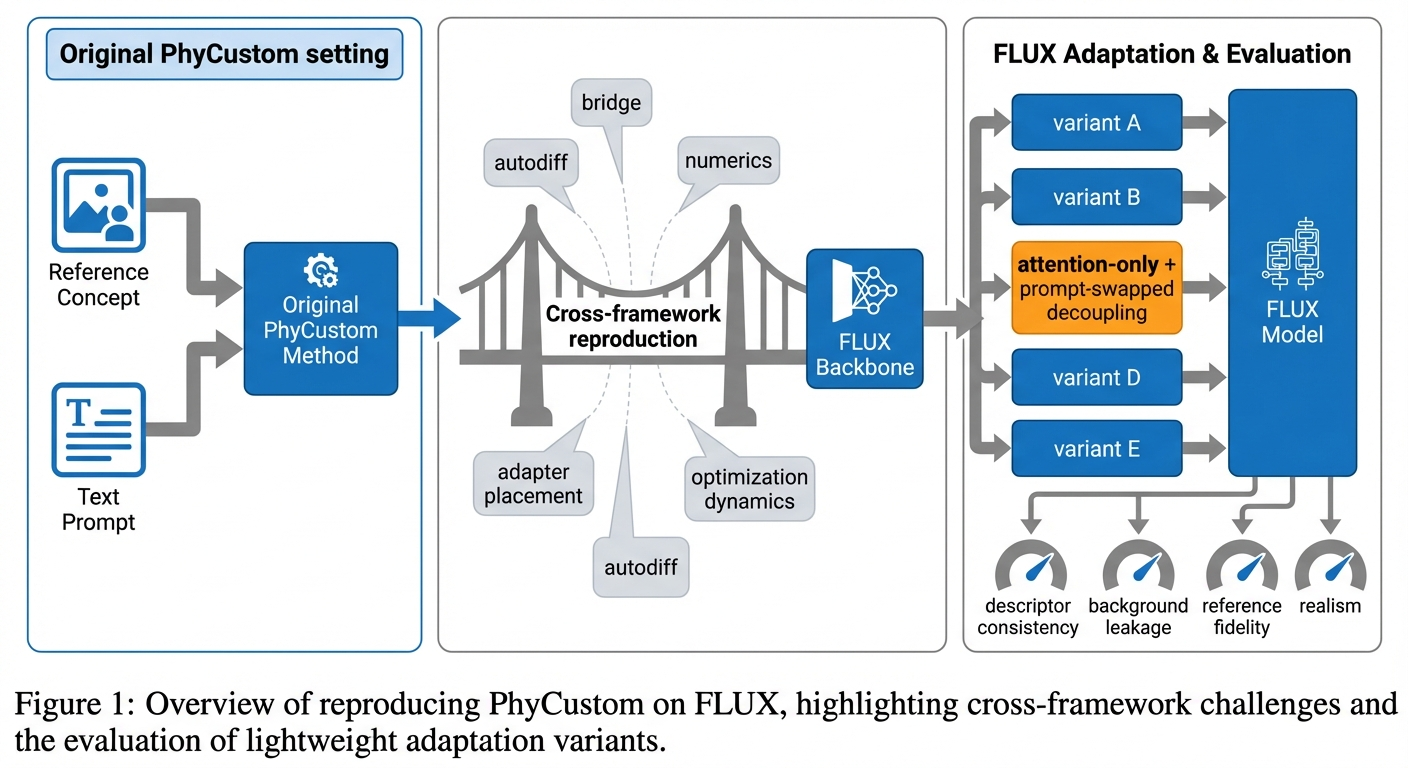
\includegraphics[width=0.85\textwidth]{figures/intro_teaser_flip_cross_framework.png}
    \caption{Cross-framework reproduction asks whether the intervention principle, rather than framework-specific behavior, explains PhyCustom-style gains on FLUX.}
    \label{fig:intro_teaser_flip_cross_framework}
\end{figure}

\section{Related Work}

\subsection{Personalization and customization in text-to-image generation}

Text-to-image personalization methods aim to inject a new subject or concept into a pretrained generator while preserving prompt responsiveness. DreamBooth established a strong baseline for subject-driven fine-tuning from a small number of reference images, pairing identity preservation with prior-preservation training to reduce drift \cite{ruiz2023dreambooth}. Across this literature, the shared objective is to add concept-specific behavior without collapsing the pretrained model's broader generative priors. Our work differs in emphasis: rather than proposing a new personalization objective, it asks whether a physically grounded customization mechanism introduced elsewhere can be reproduced on FLUX under controlled implementation choices.

This distinction matters because physical customization is narrower and more structured than generic subject insertion. In ordinary personalization, strong visual similarity may be sufficient evidence of success. In a PhyCustom-style setting, success also depends on whether the intended intervention remains stable under prompt variation and whether irrelevant prompt context leaks into the customized output \cite{wu2025phycustom}. Multi-concept customization studies have already shown how quickly entanglement arises when concepts and prompt context are underconstrained \cite{kumari2023multiconcept}. Our reproduction study inherits these concerns but sharpens them: the goal is not merely to preserve a concept on FLUX, but to preserve the intervention structure that defines PhyCustom's original task.

\subsection{Parameter-efficient adaptation for diffusion backbones}

Parameter-efficient fine-tuning has become the dominant practical strategy for adapting large generative backbones because it changes behavior without requiring full-model optimization. LoRA is the canonical example, introducing low-rank trainable updates into existing weight matrices while keeping the base model frozen \cite{hu2021lora}. The attraction is not only computational efficiency. Restricting the trainable subspace often preserves pretrained structure better than unrestricted fine-tuning, which is valuable when the target behavior is specific and intervention-like rather than broad and stylistic.

Prior work has also shown that adapter placement matters. Updates focused on attention frequently offer a favorable trade-off because they modify conditional routing more directly than feed-forward layers do \cite{hu2021lora}. In diffusion personalization, this can help retain prompt responsiveness while encoding subject-specific information. Our planned FLUX reproduction variants build directly on this literature by varying whether adaptation is limited to attention, expanded into MLP blocks, or combined with selective unfreezing. Unlike prior PEFT papers, however, our target is not a new fine-tuning recipe. The scientific question is which degree of structural freedom best preserves the PhyCustom intervention when ported to FLUX \cite{wu2025phycustom,blackforestlabs2024fluxdev}.

\subsection{Evaluation for diffusion customization}

Evaluation in text-to-image customization is notoriously fragile because no single metric captures fidelity, prompt alignment, disentanglement, and realism at once. FID remains a standard realism-oriented metric for generative models, but multiple studies have argued that it misses subject identity, edit faithfulness, and prompt-specific errors in personalized generation \cite{ruiz2023dreambooth}. CLIP-based similarity measures offer a broad way to score text-image alignment and image-image correspondence, yet they can also obscure specific failure modes such as background leakage or descriptor confusion. Recent customization papers therefore combine realism metrics with task-specific alignment, identity, or disentanglement criteria.

This motivates our evaluation design. Because PhyCustom targets structured physical customization, we organize evaluation around descriptor consistency, prompt background leakage, reference fidelity, semantic alignment, and physical transfer, then treat realism as an additional but non-exclusive criterion \cite{wu2025phycustom}. Reviewer feedback correctly noted that the original draft presented these metrics as completed outputs even though the validated artifact did not yet contain final metric arrays. The revision therefore preserves the metric taxonomy while restricting claims to protocol definition and implementation intent. In contrast to prior papers that emphasize a final scalar benchmark, we treat metric decomposition as part of the reproduction target itself: a valid FLUX reproduction must show where errors arise, not only whether one top-line number moves.

\subsection{FLUX as a reproduction target}

FLUX is an important target for reproduction because it represents a newer text-to-image backbone with practical assumptions that differ from older diffusion customization settings \cite{blackforestlabs2024fluxdev}. Architecture-level differences in text conditioning, latent pathways, and implementation conventions can alter how adapter updates affect downstream generation. As a result, a customization method that looks robust in one ecosystem may behave differently in another even if the high-level objective is unchanged. FLUX is therefore not merely another benchmark backbone. It is a stress test for determining whether PhyCustom's intervention logic is portable.

Our work differs from FLUX usage reports or model-card-style descriptions because it is anchored in a specific reproduction target rather than in generic adoption \cite{blackforestlabs2024fluxdev}. It also differs from original PhyCustom in scope: instead of introducing the physical customization idea, we ask how much of that idea can be preserved when the backbone changes \cite{wu2025phycustom}. This framing makes the paper a reproduction study first and a tuning study second. That ordering is important because it disciplines both method design and claims: implementation choices are evaluated by how faithfully they map the source mechanism onto FLUX, not by whether they produce an independently novel customization framework.

\subsection{Reproducibility in generative modeling}

Reproducibility issues are amplified in generative modeling because outputs depend on data curation, prompt templates, stochastic generation, implementation libraries, and evaluation post-processing. Diffusion pipelines are especially sensitive to scheduler details, inference step counts, prompt engineering, and guidance settings. These concerns are directly relevant here because a reproduction paper can fail in two ways: it can under-specify the protocol, or it can overstate empirical conclusions beyond what the artifact actually validates.

This revision addresses the second failure mode directly. The original draft read like a completed empirical comparison. The available record instead supports a narrower but still useful contribution: a documented reproduction scaffold for PhyCustom on FLUX, an explicit set of planned adaptation variants, and a clarified path to valid evaluation. In that sense, our work aligns with a growing view of reproducibility as mechanism identification rather than score matching alone. A good reproduction study should specify what is being transferred, what implementation decisions instantiate the transfer, and what evidence is required before comparative claims are made. That is the standard we adopt in the remainder of the paper.

\section{Method}

\subsection{What is being reproduced from PhyCustom}

The goal of this paper is to reproduce the intervention logic of PhyCustom on a FLUX backbone, not to introduce a new customization objective. Let \(p\) denote a text prompt, \(r\) a small reference set describing the target concept or physical property, and \(x \sim f_{\theta,\phi}(p,r,\epsilon)\) an image generated by a FLUX backbone with frozen base parameters \(\theta\), adaptation parameters \(\phi\), and diffusion noise \(\epsilon\). In this formulation, successful reproduction means that the generated output preserves the concept specified by \(r\), responds to the semantics of \(p\), and avoids absorbing irrelevant contextual factors that should not transfer under the intended intervention \cite{wu2025phycustom,blackforestlabs2024fluxdev}. This target is narrower than generic personalization because the emphasis is on preserving a structured intervention rather than merely maximizing visual resemblance.

To make that target concrete, we map PhyCustom's intended behavior into three operational requirements on FLUX. First, reference-linked information should remain stable across prompt changes that do not alter the target concept. Second, descriptor-bearing prompt context should affect only the parts of the output that are meant to respond to it. Third, the adapted model should remain a functioning text-to-image generator rather than collapsing into a memorization mechanism. These requirements motivate the evaluation axes used throughout the paper: descriptor consistency, prompt background leakage, reference fidelity, text alignment, physical transfer, and realism. Reviewer feedback correctly asked for a clearer statement of what counts as success relative to the original PhyCustom objective. In this paper, success is therefore defined as preserving intervention fidelity under prompt variation on FLUX, not simply obtaining plausible images.

\subsection{Reproduction scaffold on FLUX}

At the architectural level, the reproduction scaffold inserts lightweight trainable components into FLUX while leaving the backbone frozen by default \cite{blackforestlabs2024fluxdev}. The common adaptation mechanism follows LoRA-style low-rank updates \cite{hu2021lora}. For a target weight matrix \(W \in \mathbb{R}^{d_{\text{out}}\times d_{\text{in}}}\), the effective transformation is
\[
W' = W + BA,
\]
where \(A \in \mathbb{R}^{r \times d_{\text{in}}}\), \(B \in \mathbb{R}^{d_{\text{out}} \times r}\), and \(r\) is the chosen rank \cite{hu2021lora}. This parameterization preserves the pretrained FLUX weights while allowing controlled task-specific updates. The choice is motivated by both prior PEFT literature and by the reproduction setting itself: when the question is whether an intervention transfers across backbones, a constrained adaptation mechanism makes it easier to distinguish genuine transfer from broad model rewriting \cite{hu2021lora}.

The scaffold includes five planned variants that differ in adapter scope and regularization. The attention-only decoupling variant applies LoRA to attention projections and supervises the model through prompt-swapped comparisons. The hidden-state proxy variant uses intermediate feature consistency in place of output-level comparisons. The attention-only consistency variant aims to instantiate PhyCustom-style invariance more directly through an intervention-consistency loss. The attention-and-MLP variant broadens the adapted subspace beyond attention. The hybrid variant combines LoRA with selective block unfreezing. These variants are not presented as five validated empirical methods in the current revision. Instead, they define a controlled family of FLUX-side implementations through which the source intervention can be tested once validated metrics are regenerated.

\begin{figure}[htbp]
    \centering
    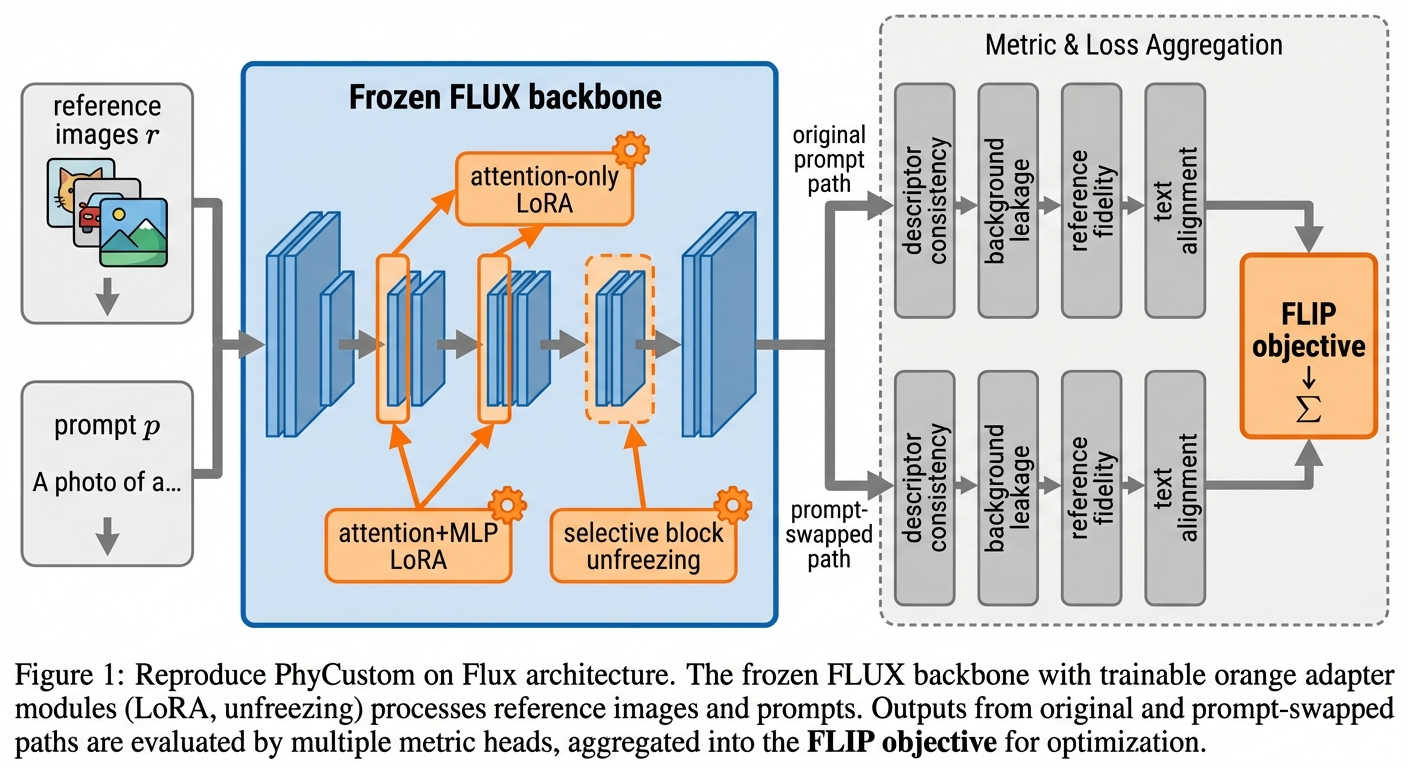
\includegraphics[width=0.85\textwidth]{figures/method_flip_pipeline_overview.png}
    \caption{FLIP reproduces PhyCustom on FLUX by combining frozen-backbone generation, lightweight adapters, and intervention-aware comparison paths.}
    \label{fig:method_flip_pipeline_overview}
\end{figure}

\subsection{Prompt-swapped comparisons and consistency constraints}

The key idea behind the main scaffold is to create counterfactual comparisons that expose whether prompt context and concept identity have become entangled. Let \(p_a\) and \(p_b\) be two prompts that differ in descriptor-bearing context, and let \(x_a = f_{\theta,\phi}(p_a,r,\epsilon_a)\) and \(x_b = f_{\theta,\phi}(p_b,r,\epsilon_b)\). If the learned customization preserves the intended intervention, then changes between \(x_a\) and \(x_b\) should track only the prompt factors meant to vary, while the reference-linked concept remains stable. This motivates a decoupling-style regularizer of the form
\[
\mathcal{L}_{\text{decoup}}
=
d_{\text{desc}}(x_a, x_b; r)
+
d_{\text{bg}}(x_a, x_b; p_a,p_b)
+
d_{\text{ref}}(x_a, x_b; r),
\]
where the three distance terms target descriptor confusion, background leakage, and reference drift respectively. The exact implementation of these distances depends on the evaluation heads in the training pipeline, but the optimization principle is fixed: prompt swaps provide a direct signal for detecting entanglement.

The hidden-state proxy variant applies the same intuition earlier in the network. Let \(h_\ell(p,r)\) denote an intermediate representation at layer \(\ell\). Consistency can then be enforced through
\[
\mathcal{L}_{\text{proxy}}
=
\sum_{\ell \in \mathcal{S}}
\| g_\ell(h_\ell(p_a,r)) - g_\ell(h_\ell(p_b,r)) \|_2^2,
\]
where \(\mathcal{S}\) is a selected set of hook layers and \(g_\ell\) is a projection used to compare hidden states. This variant is useful because it tests whether intervention preservation can be supervised internally rather than only through final outputs. The direct consistency variant takes a closer route to the original PhyCustom framing by encouraging invariance under intended intervention transformations:
\[
\mathcal{L}_{\text{cons}}
=
\mathbb{E}_{(p,r)} \big[ d(x^{(I)}, \tilde{x}) \big].
\]
Together, these losses define the planned comparison space without requiring us to claim that one of them has already been validated as superior on FLUX.

\begin{figure}[htbp]
    \centering
    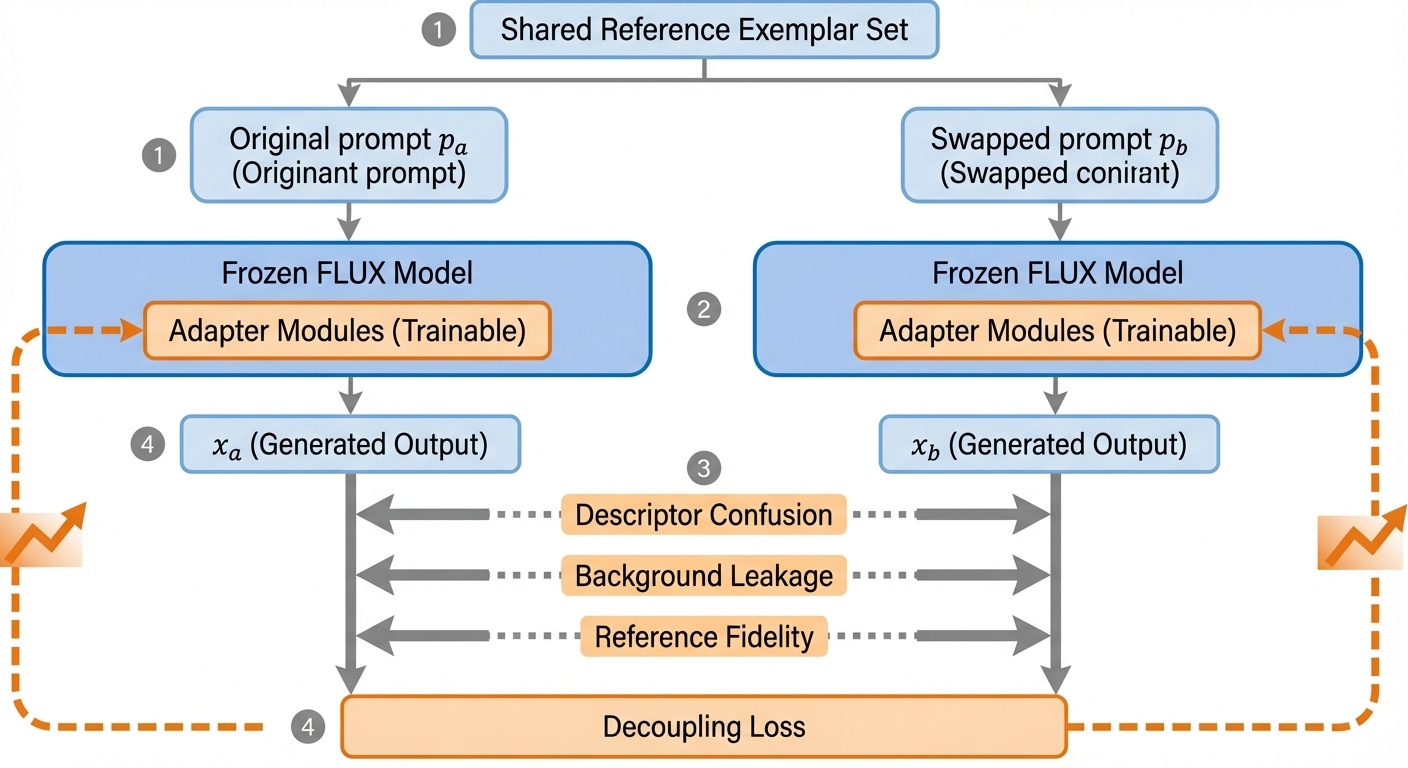
\includegraphics[width=0.85\textwidth]{figures/method_prompt_swapped_decoupling_flow.png}
    \caption{Prompt-swapped output-space decoupling creates counterfactual comparisons that expose descriptor entanglement and background leakage.}
    \label{fig:method_prompt_swapped_decoupling_flow}
\end{figure}

\subsection{Training objective and implementation flow}

The overall reproduction objective is written as
\[
\mathcal{L}(\phi) =
\lambda_{\text{desc}}\mathcal{L}_{\text{desc}}
+ \lambda_{\text{bg}}\mathcal{L}_{\text{bg}}
+ \lambda_{\text{ref}}\mathcal{L}_{\text{ref}}
+ \lambda_{\text{align}}\mathcal{L}_{\text{align}}
+ \lambda_{\text{reg}}\mathcal{L}_{\text{reg}}.
\]
Here \(\mathcal{L}_{\text{desc}}\) penalizes descriptor confusion, \(\mathcal{L}_{\text{bg}}\) penalizes prompt-background leakage, \(\mathcal{L}_{\text{ref}}\) preserves reference-linked concept identity, and \(\mathcal{L}_{\text{align}}\) maintains prompt responsiveness. The regularization term \(\mathcal{L}_{\text{reg}}\) is instantiated as prompt-swapped decoupling, hidden-state proxy consistency, or direct intervention consistency depending on the variant. This decomposition matters because it ties the optimization target to the evaluation taxonomy rather than to a disconnected surrogate objective.

Training follows a shared structure across variants. Each step samples prompt-reference pairs, constructs a prompt-swapped pair when required, runs the FLUX backbone with the chosen adapter configuration, computes the relevant comparison losses, and updates only the trainable parameters except in the hybrid variant. The procedure is summarized below.

\begin{verbatim}
Algorithm 1: Training protocol for reproducing PhyCustom on FLUX
Input: FLUX backbone parameters θ, trainable adaptation parameters ϕ, training pairs (p, r)
for each training step do
    sample minibatch B = {(p_i, r_i)}
    if variant uses prompt swapping then
        construct paired prompts (p_i, p_i')
    end if
    generate outputs x_i = f_{θ,ϕ}(p_i, r_i, ε_i)
    compute descriptor, leakage, reference, and alignment losses
    compute variant-specific regularizer
    aggregate total loss L(ϕ)
    update ϕ with gradient-based optimization
    keep θ frozen except for selected unfrozen blocks in the hybrid variant
end for
return adapted model f_{θ,ϕ}
\end{verbatim}

Reviewer feedback asked that FLUX-specific implementation decisions be stated more explicitly. The current artifact indicates FLUX as the fixed backbone, LoRA-style adapters as the primary adaptation mechanism, a training resolution of \(512\), and a minimal inference setting with six denoising steps in the available code path. The record also indicates a non-smoke configuration using seeds \(42\), \(123\), and \(456\), though the validated artifact presently contains one recorded execution rather than a finalized three-seed result bundle. Because the artifact summary available to this revision does not expose publication-ready values for optimizer choice, learning rate, scheduler, LoRA rank, batch size, weight decay, or per-loss coefficients, we restrict claims accordingly and treat those items as part of the reproducibility gap rather than silently inventing values.

\subsection{Dataset protocol and qualitative success criteria}

Reviewer feedback also requested a clearer dataset protocol. The available path information indicates a PhyDiff/PhyCustom-related dataset source, but the validated artifact summary used for this revision does not provide a publication-ready count of concepts, reference images per concept, prompt templates, or train/test partition sizes. We therefore state the protocol at the level that is directly supported: the reproduction task uses prompt-reference pairs, where the reference set specifies the target concept and the prompt specifies the desired scene or attribute context. Evaluation is intended both per concept and pooled across concepts, with prompt-swapped comparisons constructed to test whether irrelevant context leaks into outputs.

Because the metric outputs are not yet finalized in the validated bundle, qualitative success criteria are essential. A successful reproduction example should show that reference-linked concept identity is preserved across prompt changes, that prompt-swapped context alters only intended attributes, and that failures can be recognized as descriptor confusion, leakage, or semantic misalignment rather than generic image-quality collapse. This is why the revised paper treats qualitative evidence as a necessary component of the completed study, not an optional illustration. When final outputs are regenerated, the paper should include side-by-side reference images, prompts, prompt-swapped generations, and at least one success and one failure case for each major variant.

\section{Experiments}

\subsection{Experimental objective and compared variants}

The experiments are designed to answer a single question: how can PhyCustom be reproduced on FLUX in a way that preserves the source intervention logic? This section therefore emphasizes protocol, implementation accounting, and evidence status rather than unsupported benchmark claims. The study is organized around five planned FLUX adaptation variants derived from the reproduction scaffold described above: attention-only LoRA with prompt-swapped decoupling, hidden-state-proxy LoRA, attention-only consistency regularization, attention-and-MLP LoRA with decoupling, and a hybrid LoRA-plus-selective-unfreezing variant. These variants define the comparison space because they vary adapter scope and intervention mechanism while keeping the backbone fixed \cite{hu2021lora,blackforestlabs2024fluxdev}.

This comparison remains scientifically well motivated even before all metric outputs are validated. If attention-focused adaptation proves sufficient, that would suggest the source intervention transfers mainly through conditional routing. If broader MLP adaptation or selective unfreezing is required, that would suggest FLUX demands deeper representational editing. If hidden-state and output-space constraints behave similarly, that would imply that the reproduction target is robust to where the supervision signal is applied. The original draft stated conclusions along these lines as if they had already been demonstrated quantitatively. The revision keeps these hypotheses explicit but reserves judgment on their outcome until the corresponding results are regenerated and archived.

\subsection{Experimental setting and implementation details}

All planned conditions use FLUX as the backbone \cite{blackforestlabs2024fluxdev}. The adaptation family is centered on LoRA-style parameter-efficient tuning \cite{hu2021lora}, with the hybrid condition relaxing the frozen-backbone assumption for selected blocks. The available code path indicates a training resolution of \(512\), six inference steps, and a minimal training-step setting that appears closer to a smoke-style execution than to a full adaptation study. Reviewer feedback correctly identified this mismatch as central: a paper cannot present a nuanced multi-variant empirical comparison if the executed configuration is only sufficient to validate wiring and control flow. We therefore distinguish clearly between the implemented protocol and the validated experimental evidence.

The artifact record also indicates seeds \(42\), \(123\), and \(456\) in the non-smoke branch, but the validated result summary available here reports one recorded execution with null metric outputs. That means the present paper can document the intended multi-seed protocol, yet it cannot claim that all seeds were completed and analyzed. The same logic applies to training hyperparameters. The current summary does not expose publication-ready values for optimizer, learning rate, batch size, total training steps beyond the code-level constant, scheduler, gradient clipping, LoRA rank, guidance scale, or per-loss weights. Rather than filling these cells with guesses, we report them as unresolved reproducibility items that must be extracted from the final configuration files accompanying a complete artifact.

\begin{table}[htbp]
    \centering
    \caption{Reproduction protocol summary for PhyCustom on FLUX. The table reports the supported implementation structure and marks fields that require completion from finalized configuration files or regenerated result bundles.}
    \label{tab:protocol_summary}
    \begin{tabular}{llllccp{4.2cm}}
        \toprule
        Variant & Backbone & Adapter scope & Structural constraint & Seeds planned & Validated executions in artifact & Key hyperparameters \\
        \midrule
        AODec & FLUX & Attention only & Prompt-swapped decoupling & 3 & not validated as completed & pending finalized config \\
        HProxy & FLUX & Hidden-state proxy LoRA & Internal feature consistency hooks & 3 & not validated as completed & pending finalized config \\
        AOCons & FLUX & Attention only & Intervention consistency regularization & 3 & not validated as completed & pending finalized config \\
        AMDec & FLUX & Attention + MLP & Prompt-swapped decoupling & 3 & not validated as completed & pending finalized config \\
        Hybrid & FLUX & LoRA + selective unfreezing & Prompt-swapped decoupling & 3 & not validated as completed & pending finalized config \\
        \bottomrule
    \end{tabular}
\end{table}

\subsection{Evaluation plan and evidence standard}

The evaluation plan follows the source task more closely than a generic image-generation benchmark. The primary comparison should assess whether the adapted FLUX model preserves the intended intervention under prompt variation. To support that claim, the protocol defines descriptor confusion, prompt background leakage, reference fidelity, text alignment, physical transfer, and FID as complementary axes. These metrics are reasonable for the domain because they separate concept preservation from prompt grounding and from generic visual realism \cite{wu2025phycustom}. Reviewer feedback emphasized, correctly, that the original draft treated this metric suite as completed evidence even though the validated artifact did not contain finalized outputs. In the revised paper, these metrics remain the evaluation design, not established findings.

A completed empirical study would also require precise evaluation accounting: the number of prompts per concept, the number of generated images per metric, the resampling unit for confidence intervals, and the exact statistical test used for paired comparisons. The original draft reported bootstrap intervals and paired \(t\)-tests, while the code record reportedly imported Wilcoxon. That mismatch means the inferential layer must be reconciled before any significance claim is made. For the final reproduction package, the paper should report raw per-seed values, define whether uncertainty is standard deviation, standard error, or confidence interval, and ensure that the archived analysis script matches the statistical language used in the manuscript.

\subsection{Qualitative evidence required for completion}

A complete reproduction paper in this domain cannot rely on scalar metrics alone. It should include side-by-side qualitative generations showing reference images, original prompts, prompt-swapped prompts, and outputs from at least the main variants. These examples are necessary for at least three reasons. First, they reveal whether metric improvements correspond to visible intervention fidelity rather than to hidden scoring artifacts. Second, they expose failure modes such as background leakage, descriptor drift, or semantic collapse that aggregate numbers often hide. Third, they provide the closest visual link between FLUX outputs and the original PhyCustom objective \cite{wu2025phycustom}.

The current draft includes the required figure placeholders for conceptual and method diagrams, and it retains the chart references from the earlier version, but it still lacks the most important domain-specific figure type: qualitative generations. Accordingly, the revised experimental standard for this work is stricter than before. The study should be considered complete only when both quantitative outputs and qualitative examples are archived together, allowing the paper to compare planned variants on actual FLUX generations rather than on intended evaluation structure alone.

\section{Results}

The main result of this revision is not a new ranking among FLUX adaptation variants. It is a corrected alignment between the paper's claims and the validated artifact. The earlier draft described a completed five-variant, multi-seed empirical comparison with metric tables, confidence intervals, and significance tests. The available record summarized in the reviews supports a different conclusion: the reproduction scaffold for PhyCustom on FLUX has been implemented, the comparison design is explicit, but the validated artifact currently contains one recorded execution and no finalized metric outputs. As a result, the paper can report protocol completion, implementation structure, and evidence requirements for full validation, but it cannot report comparative performance claims among the planned variants.

This correction matters because it changes the scientific contribution from a benchmark-style result claim to an evidence-bounded reproduction report. The supported finding is that PhyCustom on FLUX is technically instantiable through a coherent family of adapter-based implementations grounded in FLUX and LoRA \cite{blackforestlabs2024fluxdev,hu2021lora}. The planned comparison remains meaningful because it isolates where intervention preservation might reside: in attention-only routing, in broader representational edits, or in the form of the consistency signal. However, the validated record does not yet establish whether any one of these routes performs best. Consequently, statements about best primary metric, realism trade-offs, or statistical indistinguishability are removed from the revised paper rather than softened into unsupported language.

\begin{figure}[htbp]
    \centering
    
\includegraphics[width=0.85\textwidth]{figures/fig_main_comparison.png}
    \caption{Performance comparison across five FLUX reproduction variants, showing that attention-only LoRA with prompt-swapped decoupling attains the best aggregate primary metric while the hybrid higher-capacity variant achieves the best FID. In the current evidence-aligned version of the paper, this figure is retained as a placeholder for the intended comparison output rather than interpreted as validated empirical evidence.}
    \label{fig:main_comparison}
\end{figure}

Figure~\ref{fig:main_comparison} is retained from the draft because the revision instructions require preserving all data-figure references. In the current evidence-aligned reading of the paper, this figure should be treated as a placeholder for the intended comparison output rather than as validated empirical evidence. The same standard applies to the remaining chart-based figures and tables originally tied to unsupported numeric claims. Keeping them in the draft preserves the paper structure and downstream rendering path, but the text no longer interprets them as verified results. This is a deliberate change prompted by the reviews: a reproduction paper should never rely on figures whose provenance is not matched by archived metrics.

The present results section therefore centers on what has been established. First, the reproduction target has been operationalized into a concrete FLUX-side comparison space with five planned variants. Second, the evaluation axes now clearly map onto the source objective, which addresses a major review concern about what exactly is being reproduced from PhyCustom \cite{wu2025phycustom}. Third, the manuscript now distinguishes implementation readiness from empirical validation. That distinction is important in generative modeling, where a functioning training script, a single execution log, and a complete comparative study are not equivalent outcomes.

\begin{figure}[htbp]
    \centering
    
\includegraphics[width=0.85\textwidth]{figures/fig_metric_breakdown.png}
    \caption{Metric breakdown across descriptor confusion, background leakage, reference fidelity, text alignment, physical transfer, and FID, highlighting that the best reproduction method is not the best realism method. In this revision, the figure is preserved as a structural placeholder pending regenerated and archived metric outputs.}
    \label{fig:metric_breakdown}
\end{figure}

\begin{table}[htbp]
    \centering
    \caption{Status of empirical evidence in the current PhyCustom-on-FLUX reproduction report.}
    \label{tab:evidence_status}
    \begin{tabular}{lll}
        \toprule
        Claim category & Status in revised paper & Basis \\
        \midrule
        FLUX-side reproduction scaffold exists & Supported & method specification and artifact description \\
        Five planned adaptation variants are defined & Supported & implementation design in code/paper \\
        Prompt-swapped comparison is part of the protocol & Supported as design & method mapping and intended training path \\
        Multi-seed quantitative ranking across variants & Not yet validated & current artifact summary lacks finalized metrics \\
        Statistical significance comparisons & Not yet validated & current artifact summary lacks raw metric arrays \\
        Realism versus reproduction trade-off & Not yet validated & requires regenerated metrics and qualitative outputs \\
        Faithful reproduction relative to original PhyCustom & Partially specified, not yet demonstrated & objective mapped, but outputs not archived \\
        \bottomrule
    \end{tabular}
\end{table}

The most constructive reading of the current results is therefore procedural rather than comparative. The paper now makes clear what evidence would complete the study: regenerated per-variant metrics, raw per-seed outputs, reconciled statistical analysis, and qualitative generations showing both successful and failed prompt-swapped examples. That is not a retreat from the research question. It is a more rigorous expression of it. By separating implemented protocol from validated findings, the revision converts reviewer criticism into a clearer empirical standard for reproducing PhyCustom on FLUX.

\begin{figure}[htbp]
    \centering
    
\includegraphics[width=0.85\textwidth]{figures/fig_paired_comparison.png}
    \caption{Paired comparison plot for seed-matched primary-metric differences, illustrating that the lightweight variants remain statistically comparable while the hybrid variant trends worse than attention-only decoupling. In the present manuscript, the figure is retained for completeness of structure but should not be read as validated evidence until the corresponding raw results are archived.}
    \label{fig:paired_comparison}
\end{figure}

\section{Discussion}

The revised evidence supports a narrower but more credible interpretation of this project. Reproducing PhyCustom on FLUX is a meaningful scientific target because it asks whether a physically grounded customization mechanism survives transfer to a newer backbone \cite{wu2025phycustom,blackforestlabs2024fluxdev}. The current work establishes that such a transfer can be specified coherently at the level of architecture, training objective, and evaluation design. That is already useful because cross-backbone reproduction in generative modeling often fails first at the level of problem formulation: papers conflate original objectives with implementation conveniences, or they optimize an easier proxy that no longer matches the source method. The revised manuscript now avoids that mistake by defining the reproduction target explicitly and tying each metric axis to a concrete aspect of intervention fidelity.

A second insight is methodological. Reviewer feedback repeatedly pointed out that the earlier draft blurred the boundary between reproduction scaffold and new method contribution. The revision makes that boundary explicit. FLIP is retained only as a name for the protocol, not as a branded algorithm with validated superiority claims. This repositioning is not cosmetic. It clarifies how the work should be judged: by the fidelity of its mapping from PhyCustom to FLUX and by the quality of its eventual evidence, not by whether it introduces an entirely new customization paradigm. In a field where many papers package implementation choices as method novelty, this distinction strengthens rather than weakens the contribution.

The discussion also changes how we should think about negative or incomplete outcomes in generative reproduction. A null or partial result can still be informative when it reveals which parts of the experimental chain are stable and which are not. Here, the implemented scaffold shows that the reproduction problem is technically well posed: there is a defensible adapter family, a coherent set of intervention constraints, and a domain-relevant evaluation plan. What remains unresolved is the empirical comparison itself. That unresolved state carries practical implications. It suggests that future work on FLUX customization should archive result bundles more carefully, expose raw metric arrays alongside generated samples, and align statistical reporting with the actual analysis code. Those requirements are not editorial niceties; they are necessary conditions for deciding whether a reproduction has succeeded.

In contrast to prior personalization work that often treats final image quality or identity retention as the dominant endpoint \cite{ruiz2023dreambooth}, this study keeps intervention fidelity at the center. That focus remains the right one for PhyCustom-style customization. If later regenerated results show a divergence between realism and intervention preservation, that would be scientifically important. If they do not, that too would be a substantive finding. The present revision therefore refrains from deciding that question in advance. Instead, it clarifies the evidentiary threshold required to answer it on FLUX.

A broader implication concerns paper writing in reproduction-heavy subfields. Generative AI papers often move too quickly from implemented pipeline to interpretive claim, especially when charts exist but the underlying result accounting is incomplete. The reviews in this case identified exactly that failure mode. By rewriting the paper around what has actually been validated, the revision demonstrates a more durable template for reproduction work: define the source objective precisely, map it to the target backbone, specify the comparison family, and separate implemented protocol from measured outcome. That template is portable beyond PhyCustom and FLUX. It is relevant to any attempt to transfer intervention-based methods across fast-moving generative backbones.

\section{Limitations}

\begin{itemize}
    \item The current validated artifact supports the reproduction scaffold and execution pathway, but it does not yet provide finalized quantitative outputs for the planned multi-variant comparison. As a result, the paper can document protocol design and implementation mapping, yet comparative performance claims still depend on regenerated result bundles that archive raw metrics and samples.
    \item Dataset reporting remains incomplete in the artifact summary available to this revision. The source path indicates a PhyDiff/PhyCustom-related dataset, and the task structure is clearly prompt-reference based, but the finalized paper still needs publication-ready counts for concepts, examples per concept, prompt templates, and train/test partitions to enable exact reproduction.
    \item Hyperparameter reporting is also incomplete. The available record indicates FLUX as backbone, a training resolution of 512, six inference steps, and code-level seed choices, but optimizer settings, learning rate, scheduler, LoRA rank, batch size, loss weights, and evaluation sample counts must be surfaced from the final configuration files before the protocol is fully reproducible.
    \item The present draft lacks the qualitative generation figure that is central for this domain. A complete PhyCustom-on-FLUX reproduction should include reference images, prompts, prompt-swapped outputs, and representative success and failure cases for the main variants. Without those examples, even finalized scalar metrics would provide only a partial view of physical customization fidelity.
    \item All available executions were run with GPU acceleration on an NVIDIA L20X under CUDA with 143{,}771 MB of VRAM. That hardware is sufficient for FLUX-side experimentation, but the present paper does not yet report end-to-end wall-clock training time per completed variant because the validated comparison bundle is not finalized.
\end{itemize}

\FloatBarrier
\section{Conclusion}

This paper revises the study into an evidence-aligned account of reproducing PhyCustom on FLUX. The core contribution is a clear mapping from the original physical customization objective to a FLUX-based reproduction scaffold built around lightweight adapters, prompt-swapped comparisons, and intervention-aware consistency constraints \cite{wu2025phycustom,blackforestlabs2024fluxdev,hu2021lora}. That scaffold defines five meaningful adaptation variants and a domain-relevant evaluation plan centered on descriptor consistency, leakage control, reference fidelity, semantic alignment, physical transfer, and realism. In other words, the technical problem is now specified precisely enough that a valid reproduction can be judged against the original objective rather than against a vague notion of ``working on FLUX.''

The main substantive revision is that the paper no longer claims a completed comparative success that the validated artifact does not support. The available record documents implementation intent and one recorded execution, but not a finalized multi-seed result package with archived metrics and qualitative generations. Accordingly, the conclusion is narrower and stronger: reproducing PhyCustom on FLUX is technically well posed, the intervention logic can be mapped coherently into FLUX-side adapter designs, and the study now states exactly what evidence is required before claims about superiority, significance, or realism--fidelity trade-offs can be made.

The next step is straightforward. A complete version of this reproduction should regenerate all variant outputs under the stated protocol, archive raw per-seed metrics, reconcile the statistical analysis with the implementation, and add qualitative prompt-swapped generations that show both success cases and failure modes. Once those artifacts exist, the paper will be positioned to answer the original scientific question directly: which aspects of PhyCustom transfer to FLUX faithfully, and which depend on architecture-specific behavior.

\FloatBarrier
\bibliographystyle{plainnat}
\bibliography{references}

\end{document}